% Graphic for TeX using PGF
% Title: /home/ak/git/GM_Thesis_latex/GM_Thesis/img/pareto.dia
% Creator: Dia v0.97.3
% CreationDate: Mon May 23 19:38:40 2016
% For: ak
% \usepackage{tikz}
% The following commands are not supported in PSTricks at present
% We define them conditionally, so when they are implemented,
% this pgf file will use them.
\ifx\du\undefined
  \newlength{\du}
\fi
\setlength{\du}{15\unitlength}
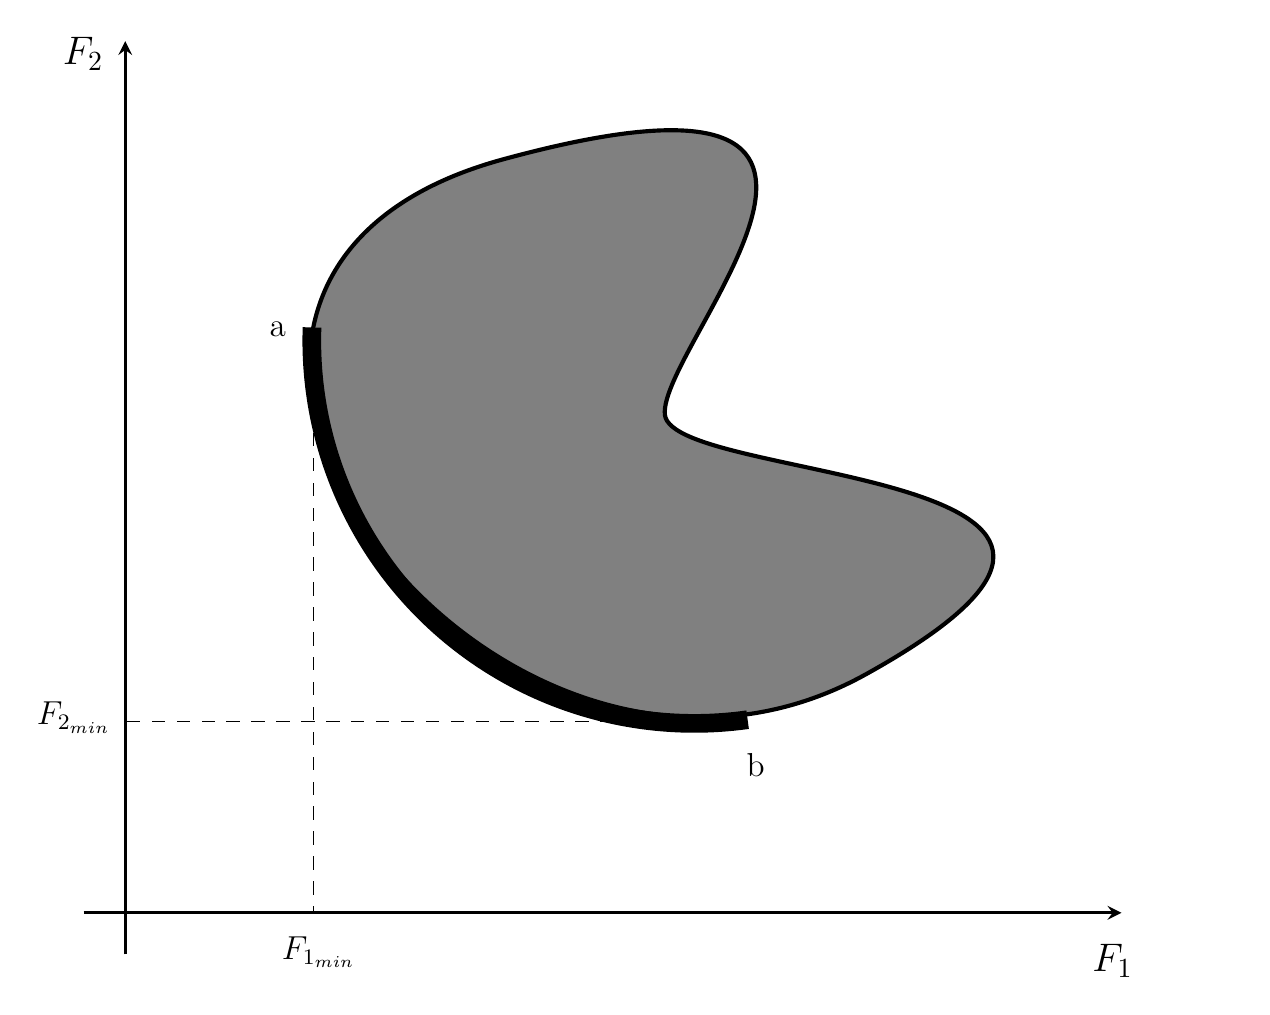
\begin{tikzpicture}
\pgftransformxscale{1.000000}
\pgftransformyscale{-1.000000}
\definecolor{dialinecolor}{rgb}{0.000000, 0.000000, 0.000000}
\pgfsetstrokecolor{dialinecolor}
\definecolor{dialinecolor}{rgb}{1.000000, 1.000000, 1.000000}
\pgfsetfillcolor{dialinecolor}
\pgfsetlinewidth{0.080000\du}
\pgfsetdash{}{0pt}
\pgfsetdash{}{0pt}
\pgfsetbuttcap
{
\definecolor{dialinecolor}{rgb}{0.000000, 0.000000, 0.000000}
\pgfsetfillcolor{dialinecolor}
% was here!!!
\pgfsetarrowsend{stealth}
\definecolor{dialinecolor}{rgb}{0.000000, 0.000000, 0.000000}
\pgfsetstrokecolor{dialinecolor}
\draw (9.000000\du,36.000000\du)--(9.000000\du,14.000000\du);
}
\pgfsetlinewidth{0.080000\du}
\pgfsetdash{}{0pt}
\pgfsetdash{}{0pt}
\pgfsetbuttcap
{
\definecolor{dialinecolor}{rgb}{0.000000, 0.000000, 0.000000}
\pgfsetfillcolor{dialinecolor}
% was here!!!
\pgfsetarrowsend{stealth}
\definecolor{dialinecolor}{rgb}{0.000000, 0.000000, 0.000000}
\pgfsetstrokecolor{dialinecolor}
\draw (8.000000\du,35.000000\du)--(33.000000\du,35.000000\du);
}
\pgfsetlinewidth{0.100000\du}
\pgfsetdash{}{0pt}
\pgfsetdash{}{0pt}
\pgfsetmiterjoin
\pgfsetbuttcap
\definecolor{dialinecolor}{rgb}{1.000000, 1.000000, 1.000000}
\pgfsetfillcolor{gray}
\pgfpathmoveto{\pgfpoint{26.850000\du}{29.250000\du}}
\pgfpathcurveto{\pgfpoint{35.850000\du}{24.250000\du}}{\pgfpoint{22.166667\du}{24.666667\du}}{\pgfpoint{22.000000\du}{23.000000\du}}
\pgfpathcurveto{\pgfpoint{21.833333\du}{21.333333\du}}{\pgfpoint{29.100000\du}{13.850000\du}}{\pgfpoint{18.100000\du}{16.850000\du}}
\pgfpathcurveto{\pgfpoint{7.100000\du}{19.850000\du}}{\pgfpoint{17.850000\du}{34.250000\du}}{\pgfpoint{26.850000\du}{29.250000\du}}
\pgfusepath{fill}
\definecolor{dialinecolor}{rgb}{0.000000, 0.000000, 0.000000}
\pgfsetstrokecolor{dialinecolor}
\pgfpathmoveto{\pgfpoint{26.850000\du}{29.250000\du}}
\pgfpathcurveto{\pgfpoint{35.850000\du}{24.250000\du}}{\pgfpoint{22.166667\du}{24.666667\du}}{\pgfpoint{22.000000\du}{23.000000\du}}
\pgfpathcurveto{\pgfpoint{21.833333\du}{21.333333\du}}{\pgfpoint{29.100000\du}{13.850000\du}}{\pgfpoint{18.100000\du}{16.850000\du}}
\pgfpathcurveto{\pgfpoint{7.100000\du}{19.850000\du}}{\pgfpoint{17.850000\du}{34.250000\du}}{\pgfpoint{26.850000\du}{29.250000\du}}
\pgfusepath{stroke}
\pgfsetlinewidth{0.450000\du}
\pgfsetdash{}{0pt}
\pgfsetdash{}{0pt}
\pgfsetbuttcap
{
\definecolor{dialinecolor}{rgb}{0.000000, 0.000000, 0.000000}
\pgfsetfillcolor{dialinecolor}
% was here!!!
\definecolor{dialinecolor}{rgb}{0.000000, 0.000000, 0.000000}
\pgfsetstrokecolor{dialinecolor}
\pgfpathmoveto{\pgfpoint{13.500010\du}{20.899518\du}}
\pgfpatharc{182}{82}{9.216322\du and 9.216322\du}
\pgfusepath{stroke}
}
% setfont left to latex
\definecolor{dialinecolor}{rgb}{0.000000, 0.000000, 0.000000}
\pgfsetstrokecolor{dialinecolor}
\node[anchor=west] at (31.850000\du,36.150000\du){\mbox{\Large $F_1$}};
% setfont left to latex
\definecolor{dialinecolor}{rgb}{0.000000, 0.000000, 0.000000}
\pgfsetstrokecolor{dialinecolor}
\node[anchor=west] at (7.050000\du,14.300000\du){\mbox{\Large $F_2$}};
\pgfsetlinewidth{0.000000\du}
\pgfsetdash{{1.000000\du}{1.000000\du}}{0\du}
\pgfsetdash{{0.300000\du}{0.300000\du}}{0\du}
\pgfsetbuttcap
{
\definecolor{dialinecolor}{rgb}{0.000000, 0.000000, 0.000000}
\pgfsetfillcolor{dialinecolor}
% was here!!!
\definecolor{dialinecolor}{rgb}{0.000000, 0.000000, 0.000000}
\pgfsetstrokecolor{dialinecolor}
\draw (9.050000\du,30.400000\du)--(24.000000\du,30.400000\du);
}
\pgfsetlinewidth{0.000000\du}
\pgfsetdash{{0.300000\du}{0.300000\du}}{0\du}
\pgfsetdash{{0.300000\du}{0.300000\du}}{0\du}
\pgfsetbuttcap
{
\definecolor{dialinecolor}{rgb}{0.000000, 0.000000, 0.000000}
\pgfsetfillcolor{dialinecolor}
% was here!!!
\definecolor{dialinecolor}{rgb}{0.000000, 0.000000, 0.000000}
\pgfsetstrokecolor{dialinecolor}
\draw (13.550000\du,21.050000\du)--(13.525000\du,34.987500\du);
}
% setfont left to latex
\definecolor{dialinecolor}{rgb}{0.000000, 0.000000, 0.000000}
\pgfsetstrokecolor{dialinecolor}
\node[anchor=west] at (12.550000\du,35.950000\du){\mbox{\large $F_{1_{min}}$}};
% setfont left to latex
\definecolor{dialinecolor}{rgb}{0.000000, 0.000000, 0.000000}
\pgfsetstrokecolor{dialinecolor}
\node[anchor=west] at (6.650000\du,30.300000\du){\mbox{\large $F_{2_{min}}$}};
% setfont left to latex
\definecolor{dialinecolor}{rgb}{0.000000, 0.000000, 0.000000}
\pgfsetstrokecolor{dialinecolor}
\node[anchor=west] at (12.250000\du,20.950000\du){\large a};
% setfont left to latex
\definecolor{dialinecolor}{rgb}{0.000000, 0.000000, 0.000000}
\pgfsetstrokecolor{dialinecolor}
\node[anchor=west] at (23.750000\du,31.450000\du){\large b};
\end{tikzpicture}
